\documentclass{article}\usepackage[]{graphicx}\usepackage[]{color}
%% maxwidth is the original width if it is less than linewidth
%% otherwise use linewidth (to make sure the graphics do not exceed the margin)
\makeatletter
\def\maxwidth{ %
  \ifdim\Gin@nat@width>\linewidth
    \linewidth
  \else
    \Gin@nat@width
  \fi
}
\makeatother

\definecolor{fgcolor}{rgb}{0.345, 0.345, 0.345}
\newcommand{\hlnum}[1]{\textcolor[rgb]{0.686,0.059,0.569}{#1}}%
\newcommand{\hlstr}[1]{\textcolor[rgb]{0.192,0.494,0.8}{#1}}%
\newcommand{\hlcom}[1]{\textcolor[rgb]{0.678,0.584,0.686}{\textit{#1}}}%
\newcommand{\hlopt}[1]{\textcolor[rgb]{0,0,0}{#1}}%
\newcommand{\hlstd}[1]{\textcolor[rgb]{0.345,0.345,0.345}{#1}}%
\newcommand{\hlkwa}[1]{\textcolor[rgb]{0.161,0.373,0.58}{\textbf{#1}}}%
\newcommand{\hlkwb}[1]{\textcolor[rgb]{0.69,0.353,0.396}{#1}}%
\newcommand{\hlkwc}[1]{\textcolor[rgb]{0.333,0.667,0.333}{#1}}%
\newcommand{\hlkwd}[1]{\textcolor[rgb]{0.737,0.353,0.396}{\textbf{#1}}}%

\usepackage{framed}
\makeatletter
\newenvironment{kframe}{%
 \def\at@end@of@kframe{}%
 \ifinner\ifhmode%
  \def\at@end@of@kframe{\end{minipage}}%
  \begin{minipage}{\columnwidth}%
 \fi\fi%
 \def\FrameCommand##1{\hskip\@totalleftmargin \hskip-\fboxsep
 \colorbox{shadecolor}{##1}\hskip-\fboxsep
     % There is no \\@totalrightmargin, so:
     \hskip-\linewidth \hskip-\@totalleftmargin \hskip\columnwidth}%
 \MakeFramed {\advance\hsize-\width
   \@totalleftmargin\z@ \linewidth\hsize
   \@setminipage}}%
 {\par\unskip\endMakeFramed%
 \at@end@of@kframe}
\makeatother

\definecolor{shadecolor}{rgb}{.97, .97, .97}
\definecolor{messagecolor}{rgb}{0, 0, 0}
\definecolor{warningcolor}{rgb}{1, 0, 1}
\definecolor{errorcolor}{rgb}{1, 0, 0}
\newenvironment{knitrout}{}{} % an empty environment to be redefined in TeX

\usepackage{alltt}
\IfFileExists{upquote.sty}{\usepackage{upquote}}{}
\begin{document}

\begin{knitrout}
\definecolor{shadecolor}{rgb}{0.969, 0.969, 0.969}\color{fgcolor}\begin{kframe}
\begin{alltt}
\hlcom{#GUIA 8}

\hlstd{Notas}\hlkwb{<-}\hlkwd{c}\hlstd{(}\hlnum{4.47}\hlstd{,}\hlnum{4.47}\hlstd{,}\hlnum{3.48}\hlstd{,}\hlnum{5.0}\hlstd{,}\hlnum{3.42}\hlstd{,}\hlnum{3.78}\hlstd{,}\hlnum{3.1}\hlstd{,}\hlnum{3.57}\hlstd{,}\hlnum{4.2}\hlstd{,}\hlnum{4.5}\hlstd{,}\hlnum{3.6}\hlstd{,}\hlnum{3.75}\hlstd{,}\hlnum{4.5}\hlstd{,}\hlnum{2.85}\hlstd{,}\hlnum{3.7}\hlstd{,}\hlnum{4.2}\hlstd{,}\hlnum{3.2}\hlstd{,}\hlnum{4.05}\hlstd{,}\hlnum{4.9}\hlstd{,}\hlnum{5.1}\hlstd{,}\hlnum{5.3}\hlstd{,}\hlnum{4.16}\hlstd{,}\hlnum{4.56}\hlstd{,}\hlnum{3.54}\hlstd{,}\hlnum{3.5}\hlstd{,}\hlnum{5.2}\hlstd{,}\hlnum{4.71}\hlstd{,}\hlnum{3.7}\hlstd{,}\hlnum{4.78}\hlstd{,}\hlnum{4.14}\hlstd{,}\hlnum{4.14}\hlstd{,}\hlnum{4.8}\hlstd{,}\hlnum{4.1}\hlstd{,}\hlnum{3.83}\hlstd{,}\hlnum{3.6}\hlstd{,}\hlnum{2.98}\hlstd{,}\hlnum{4.32}\hlstd{,}\hlnum{5.1}\hlstd{,}\hlnum{4.3}\hlstd{,}\hlnum{3.9}\hlstd{,}\hlnum{3.96}\hlstd{,}\hlnum{3.54}\hlstd{,}\hlnum{4.8}\hlstd{,}\hlnum{4.3}\hlstd{,}\hlnum{3.39}\hlstd{,}\hlnum{4.47}\hlstd{,}\hlnum{3.19}\hlstd{,}\hlnum{3.75}\hlstd{,}\hlnum{3.1}\hlstd{,}\hlnum{4.7}\hlstd{,}\hlnum{3.69}\hlstd{,}\hlnum{3.3}\hlstd{,}\hlnum{2.85}\hlstd{,}\hlnum{5.25}\hlstd{,}\hlnum{4.68}\hlstd{,}\hlnum{4.04}\hlstd{,}\hlnum{4.44}\hlstd{,}\hlnum{5.43}\hlstd{,}\hlnum{3.04}\hlstd{,}\hlnum{2.95}\hlstd{);Notas}
\end{alltt}
\begin{verbatim}
##  [1] 4.47 4.47 3.48 5.00 3.42 3.78 3.10 3.57 4.20 4.50 3.60 3.75 4.50 2.85
## [15] 3.70 4.20 3.20 4.05 4.90 5.10 5.30 4.16 4.56 3.54 3.50 5.20 4.71 3.70
## [29] 4.78 4.14 4.14 4.80 4.10 3.83 3.60 2.98 4.32 5.10 4.30 3.90 3.96 3.54
## [43] 4.80 4.30 3.39 4.47 3.19 3.75 3.10 4.70 3.69 3.30 2.85 5.25 4.68 4.04
## [57] 4.44 5.43 3.04 2.95
\end{verbatim}
\begin{alltt}
\hlkwd{data.entry}\hlstd{(Notas)}
\hlstd{Notas}
\end{alltt}
\begin{verbatim}
##  [1] 4.47 4.47 3.48 5.00 3.42 3.78 3.10 3.57 4.20 4.50 3.60 3.75 4.50 2.85
## [15] 3.70 4.20 3.20 4.05 4.90 5.10 5.30 4.16 4.56 3.54 3.50 5.20 4.71 3.70
## [29] 4.78 4.14 4.14 4.80 4.10 3.83 3.60 2.98 4.32 5.10 4.30 3.90 3.96 3.54
## [43] 4.80 4.30 3.39 4.47 3.19 3.75 3.10 4.70 3.69 3.30 2.85 5.25 4.68 4.04
## [57] 4.44 5.43 3.04 2.95
\end{verbatim}
\begin{alltt}
\hlkwd{length}\hlstd{(Notas)}
\end{alltt}
\begin{verbatim}
## [1] 60
\end{verbatim}
\begin{alltt}
\hlkwd{write}\hlstd{(Notas,} \hlstr{"Notas.txt"}\hlstd{)}
\hlkwd{ls}\hlstd{()}
\end{alltt}
\begin{verbatim}
## [1] "Notas"
\end{verbatim}
\begin{alltt}
\hlkwd{rm}\hlstd{(}\hlkwc{list}\hlstd{=}\hlkwd{ls}\hlstd{(}\hlkwc{all}\hlstd{=}\hlnum{TRUE}\hlstd{))}
\hlkwd{ls}\hlstd{()}
\end{alltt}
\begin{verbatim}
## character(0)
\end{verbatim}
\begin{alltt}
\hlstd{X} \hlkwb{<-} \hlkwd{scan}\hlstd{(}\hlstr{"Notas.txt"}\hlstd{,} \hlkwc{what} \hlstd{=} \hlkwd{double}\hlstd{(}\hlnum{0}\hlstd{),} \hlkwc{na.strings} \hlstd{=} \hlstr{"NA"}\hlstd{,} \hlkwc{flush}\hlstd{=}\hlnum{FALSE}\hlstd{)}
\hlkwd{ls}\hlstd{()}
\end{alltt}
\begin{verbatim}
## [1] "X"
\end{verbatim}
\begin{alltt}
\hlstd{n} \hlkwb{<-} \hlkwd{length}\hlstd{(X); n}
\end{alltt}
\begin{verbatim}
## [1] 60
\end{verbatim}
\begin{alltt}
\hlstd{k} \hlkwb{<-} \hlnum{1}\hlopt{+}\hlnum{3.322}\hlopt{*}\hlkwd{logb}\hlstd{(}\hlnum{60}\hlstd{,} \hlnum{10}\hlstd{); k}
\end{alltt}
\begin{verbatim}
## [1] 6.907018
\end{verbatim}
\begin{alltt}
\hlstd{k} \hlkwb{<-} \hlkwd{round}\hlstd{(k); k}
\end{alltt}
\begin{verbatim}
## [1] 7
\end{verbatim}
\begin{alltt}
\hlstd{rango} \hlkwb{<-} \hlkwd{max}\hlstd{(X)}\hlopt{-}\hlkwd{min}\hlstd{(X); rango}
\end{alltt}
\begin{verbatim}
## [1] 2.58
\end{verbatim}
\begin{alltt}
\hlstd{a}\hlkwb{=}\hlstd{rango}\hlopt{/}\hlstd{k; a}
\end{alltt}
\begin{verbatim}
## [1] 0.3685714
\end{verbatim}
\begin{alltt}
\hlstd{a} \hlkwb{<-} \hlkwd{round}\hlstd{(a,} \hlnum{3}\hlstd{); a}
\end{alltt}
\begin{verbatim}
## [1] 0.369
\end{verbatim}
\begin{alltt}
\hlstd{rango} \hlkwb{<-} \hlkwd{max}\hlstd{(X)}\hlopt{-}\hlkwd{min}\hlstd{(X); rango}
\end{alltt}
\begin{verbatim}
## [1] 2.58
\end{verbatim}
\begin{alltt}
\hlstd{a}\hlkwb{=}\hlstd{rango}\hlopt{/}\hlstd{k; a}
\end{alltt}
\begin{verbatim}
## [1] 0.3685714
\end{verbatim}
\begin{alltt}
\hlstd{a} \hlkwb{<-} \hlkwd{round}\hlstd{(a,} \hlnum{3}\hlstd{); a}
\end{alltt}
\begin{verbatim}
## [1] 0.369
\end{verbatim}
\begin{alltt}
\hlstd{limites} \hlkwb{<-} \hlkwd{seq}\hlstd{(}\hlkwc{from}\hlstd{=}\hlkwd{min}\hlstd{(X)}\hlopt{-}\hlnum{0.01}\hlopt{/}\hlnum{2}\hlstd{,} \hlkwc{to}\hlstd{=}\hlkwd{max}\hlstd{(X)}\hlopt{+}\hlnum{0.01}\hlopt{/}\hlnum{2}\hlstd{,} \hlkwc{by}\hlstd{=a); limites}
\end{alltt}
\begin{verbatim}
## [1] 2.845 3.214 3.583 3.952 4.321 4.690 5.059 5.428
\end{verbatim}
\begin{alltt}
\hlkwd{options}\hlstd{(}\hlkwc{digits}\hlstd{=}\hlnum{4}\hlstd{)}
\hlstd{ci} \hlkwb{<-} \hlkwd{cbind}\hlstd{(}\hlnum{1}\hlopt{:}\hlstd{k); ci}
\end{alltt}
\begin{verbatim}
##      [,1]
## [1,]    1
## [2,]    2
## [3,]    3
## [4,]    4
## [5,]    5
## [6,]    6
## [7,]    7
\end{verbatim}
\begin{alltt}
\hlkwa{for}\hlstd{(i} \hlkwa{in} \hlnum{2}\hlopt{:}\hlkwd{length}\hlstd{(limites)) ci[i}\hlopt{-}\hlnum{1}\hlstd{,} \hlnum{1}\hlstd{]} \hlkwb{<-} \hlstd{(limites[i]} \hlopt{+} \hlstd{limites[i}\hlopt{-}\hlnum{1}\hlstd{])}\hlopt{/}\hlnum{2}
\hlstd{ci}
\end{alltt}
\begin{verbatim}
##       [,1]
## [1,] 3.030
## [2,] 3.399
## [3,] 3.768
## [4,] 4.136
## [5,] 4.505
## [6,] 4.875
## [7,] 5.244
\end{verbatim}
\begin{alltt}
\hlkwd{options}\hlstd{(}\hlkwc{digits}\hlstd{=}\hlnum{2}\hlstd{)}
\hlstd{fi} \hlkwb{<-} \hlkwd{cbind}\hlstd{(}\hlkwd{table}\hlstd{(}\hlkwd{cut}\hlstd{(X,} \hlkwc{breaks} \hlstd{= limites,} \hlkwc{labels}\hlstd{=}\hlkwa{NULL}\hlstd{,} \hlkwc{include.lowest}\hlstd{=}\hlnum{FALSE}\hlstd{,}
\hlkwc{right}\hlstd{=}\hlnum{FALSE}\hlstd{,} \hlkwc{dig.lab}\hlstd{=}\hlnum{4}\hlstd{))); fi}
\end{alltt}
\begin{verbatim}
##               [,1]
## [2.845,3.214)    9
## [3.214,3.583)    8
## [3.583,3.952)   10
## [3.952,4.321)   12
## [4.321,4.69)     8
## [4.69,5.059)     7
## [5.059,5.428)    5
\end{verbatim}
\begin{alltt}
\hlkwd{options}\hlstd{(}\hlkwc{digits}\hlstd{=}\hlnum{4}\hlstd{)}
\hlstd{fri} \hlkwb{<-} \hlstd{fi}\hlopt{/}\hlstd{n; fri}
\end{alltt}
\begin{verbatim}
##                  [,1]
## [2.845,3.214) 0.15000
## [3.214,3.583) 0.13333
## [3.583,3.952) 0.16667
## [3.952,4.321) 0.20000
## [4.321,4.69)  0.13333
## [4.69,5.059)  0.11667
## [5.059,5.428) 0.08333
\end{verbatim}
\begin{alltt}
\hlkwd{options}\hlstd{(}\hlkwc{digits}\hlstd{=}\hlnum{2}\hlstd{)}
\hlstd{Fi} \hlkwb{<-} \hlkwd{cumsum}\hlstd{(fi); Fi}
\end{alltt}
\begin{verbatim}
## [1]  9 17 27 39 47 54 59
\end{verbatim}
\begin{alltt}
\hlkwd{options}\hlstd{(}\hlkwc{digits}\hlstd{=}\hlnum{4}\hlstd{)}
\hlstd{Fri} \hlkwb{<-} \hlstd{Fi}\hlopt{/}\hlstd{n; Fri}
\end{alltt}
\begin{verbatim}
## [1] 0.1500 0.2833 0.4500 0.6500 0.7833 0.9000 0.9833
\end{verbatim}
\begin{alltt}
\hlstd{tablaFrec} \hlkwb{<-} \hlkwd{data.frame}\hlstd{(}\hlkwc{ci}\hlstd{=ci,} \hlkwc{fi}\hlstd{=fi,} \hlkwc{fri}\hlstd{=fri,} \hlkwc{Fi}\hlstd{=Fi,} \hlkwc{Fri}\hlstd{=Fri); tablaFrec}
\end{alltt}
\begin{verbatim}
##                  ci fi     fri Fi    Fri
## [2.845,3.214) 3.030  9 0.15000  9 0.1500
## [3.214,3.583) 3.399  8 0.13333 17 0.2833
## [3.583,3.952) 3.768 10 0.16667 27 0.4500
## [3.952,4.321) 4.136 12 0.20000 39 0.6500
## [4.321,4.69)  4.505  8 0.13333 47 0.7833
## [4.69,5.059)  4.875  7 0.11667 54 0.9000
## [5.059,5.428) 5.244  5 0.08333 59 0.9833
\end{verbatim}
\begin{alltt}
\hlstd{h} \hlkwb{<-} \hlkwd{hist}\hlstd{(X,} \hlkwc{breaks}\hlstd{=}\hlkwd{c}\hlstd{(limites[}\hlnum{1}\hlstd{]}\hlopt{-}\hlstd{a, limites, limites[k}\hlopt{+}\hlnum{1}\hlstd{]}\hlopt{+}\hlstd{a),} \hlkwc{freq} \hlstd{=} \hlnum{TRUE}\hlstd{,} \hlkwc{probability} \hlstd{=} \hlnum{FALSE}\hlstd{,}
\hlkwc{include.lowest} \hlstd{=} \hlnum{FALSE}\hlstd{,}\hlkwc{right} \hlstd{=} \hlnum{TRUE}\hlstd{,} \hlkwc{main} \hlstd{=} \hlstr{"Histograma de frecuencias"}\hlstd{,}
\hlkwc{col}\hlstd{=}\hlstr{"lightyellow"}\hlstd{,} \hlkwc{lty}\hlstd{=}\hlnum{1}\hlstd{,} \hlkwc{border}\hlstd{=}\hlstr{"purple"}\hlstd{,} \hlkwc{xlab}\hlstd{=}\hlstr{" Notas de aspirantes"}\hlstd{,} \hlkwc{ylab}\hlstd{=}\hlstr{"Frecuencia (fi)"}\hlstd{,}
\hlkwc{axes}\hlstd{=}\hlnum{TRUE}\hlstd{,} \hlkwc{labels}\hlstd{=}\hlnum{FALSE}\hlstd{)}
\hlkwd{text}\hlstd{(h}\hlopt{$}\hlstd{mids, h}\hlopt{$}\hlstd{density, h}\hlopt{$}\hlstd{counts,} \hlkwc{adj}\hlstd{=}\hlkwd{c}\hlstd{(}\hlnum{0.5}\hlstd{,} \hlopt{-}\hlnum{0.5}\hlstd{),} \hlkwc{col}\hlstd{=}\hlstr{"red"}\hlstd{)}
\hlkwd{rug}\hlstd{(}\hlkwd{jitter}\hlstd{(X))} \hlcom{# adiciona marcas de los datos}
\end{alltt}
\end{kframe}
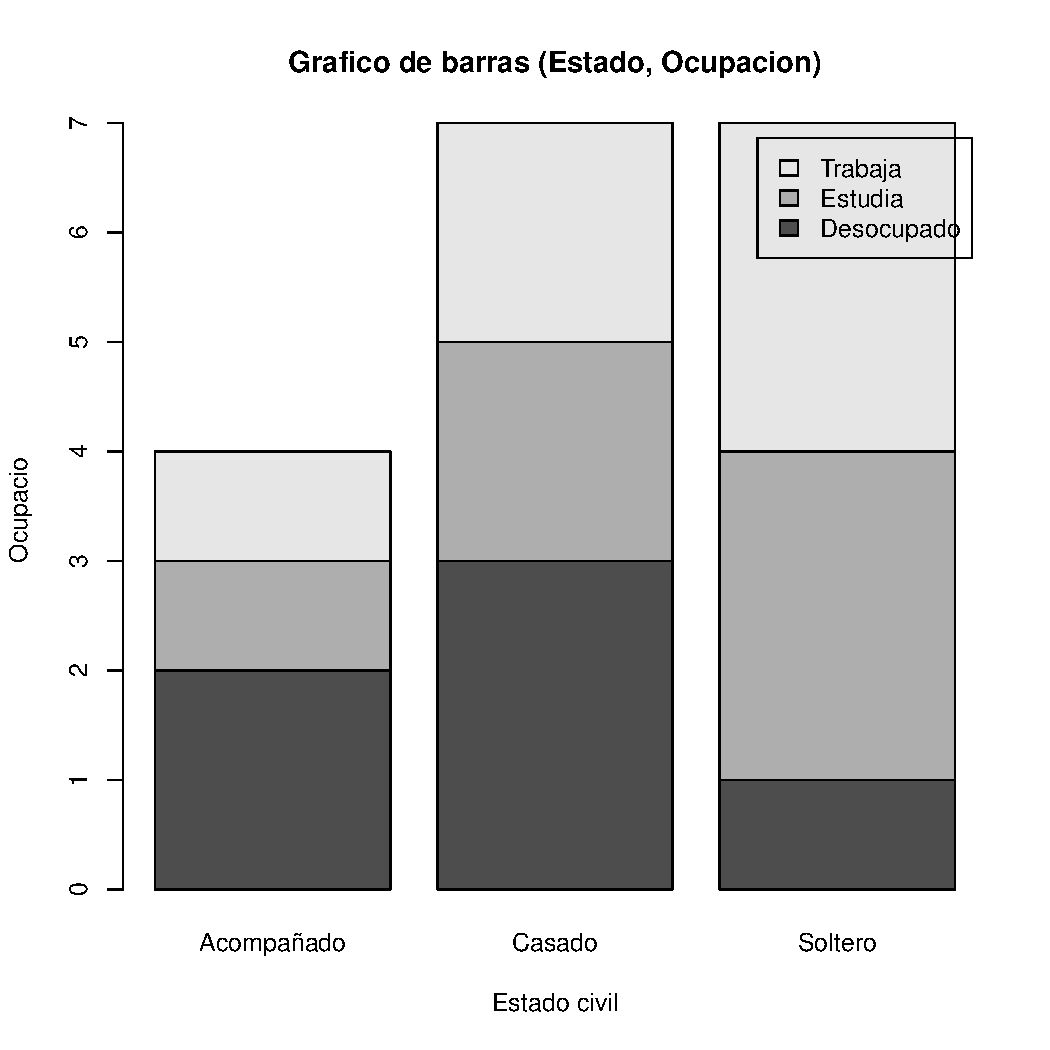
\includegraphics[width=\maxwidth]{figure/unnamed-chunk-1-1} 
\begin{kframe}\begin{alltt}
\hlkwd{is.list}\hlstd{(h); h}
\end{alltt}
\begin{verbatim}
## [1] TRUE
## $breaks
##  [1] 2.476 2.845 3.214 3.583 3.952 4.321 4.690 5.059 5.428 5.797
## 
## $counts
## [1]  0  9  8 10 12  8  7  5  1
## 
## $density
## [1] 0.00000 0.40650 0.36134 0.45167 0.54201 0.36134 0.31617 0.22584 0.04517
## 
## $mids
## [1] 2.660 3.030 3.399 3.768 4.136 4.505 4.875 5.244 5.613
## 
## $xname
## [1] "X"
## 
## $equidist
## [1] TRUE
## 
## attr(,"class")
## [1] "histogram"
\end{verbatim}
\begin{alltt}
\hlstd{h} \hlkwb{<-} \hlkwd{hist}\hlstd{(X,} \hlkwc{breaks}\hlstd{=}\hlkwd{c}\hlstd{(limites[}\hlnum{1}\hlstd{]}\hlopt{-}\hlstd{a, limites, limites[k}\hlopt{+}\hlnum{1}\hlstd{]}\hlopt{+}\hlstd{a),} \hlkwc{freq} \hlstd{=} \hlnum{FALSE}\hlstd{,}
\hlkwc{probability} \hlstd{=} \hlnum{TRUE}\hlstd{,} \hlkwc{include.lowest} \hlstd{=} \hlnum{FALSE}\hlstd{,} \hlkwc{right} \hlstd{=} \hlnum{TRUE}\hlstd{,}
\hlkwc{main}\hlstd{=}\hlstr{"Aproximacion a una Normal\textbackslash{}n"}\hlstd{,} \hlkwc{col}\hlstd{=}\hlstr{"lightyellow"}\hlstd{,}\hlkwc{lty}\hlstd{=}\hlnum{1}\hlstd{,}\hlkwc{border}\hlstd{=}\hlstr{"purple"}\hlstd{,}
\hlkwc{xlab}\hlstd{=}\hlstr{"Notas de aspirantes\textbackslash{}n"}\hlstd{,} \hlkwc{ylab}\hlstd{=}\hlstr{"Frecuencia relativa (fri)"}\hlstd{,}
\hlkwc{axes}\hlstd{=}\hlnum{TRUE}\hlstd{,} \hlkwc{labels}\hlstd{=}\hlnum{FALSE}\hlstd{)}
\hlkwd{text}\hlstd{(h}\hlopt{$}\hlstd{mids, h}\hlopt{$}\hlstd{density, h}\hlopt{$}\hlstd{counts,} \hlkwc{adj}\hlstd{=}\hlkwd{c}\hlstd{(}\hlnum{0.5}\hlstd{,} \hlnum{0.2}\hlstd{),} \hlkwc{col}\hlstd{=}\hlstr{"red"}\hlstd{)}
\hlkwd{rug}\hlstd{(}\hlkwd{jitter}\hlstd{(X))} \hlcom{# adiciona marcas de los datos}
\hlkwd{curve}\hlstd{(}\hlkwd{dnorm}\hlstd{(x,} \hlkwc{mean}\hlstd{=}\hlkwd{mean}\hlstd{(X),} \hlkwc{sd}\hlstd{=}\hlkwd{sd}\hlstd{(X)),} \hlkwc{col} \hlstd{=} \hlnum{2}\hlstd{,} \hlkwc{lty} \hlstd{=} \hlnum{2}\hlstd{,}\hlkwc{lwd} \hlstd{=} \hlnum{2}\hlstd{,} \hlkwc{add} \hlstd{=} \hlnum{TRUE}\hlstd{)}
\end{alltt}
\end{kframe}
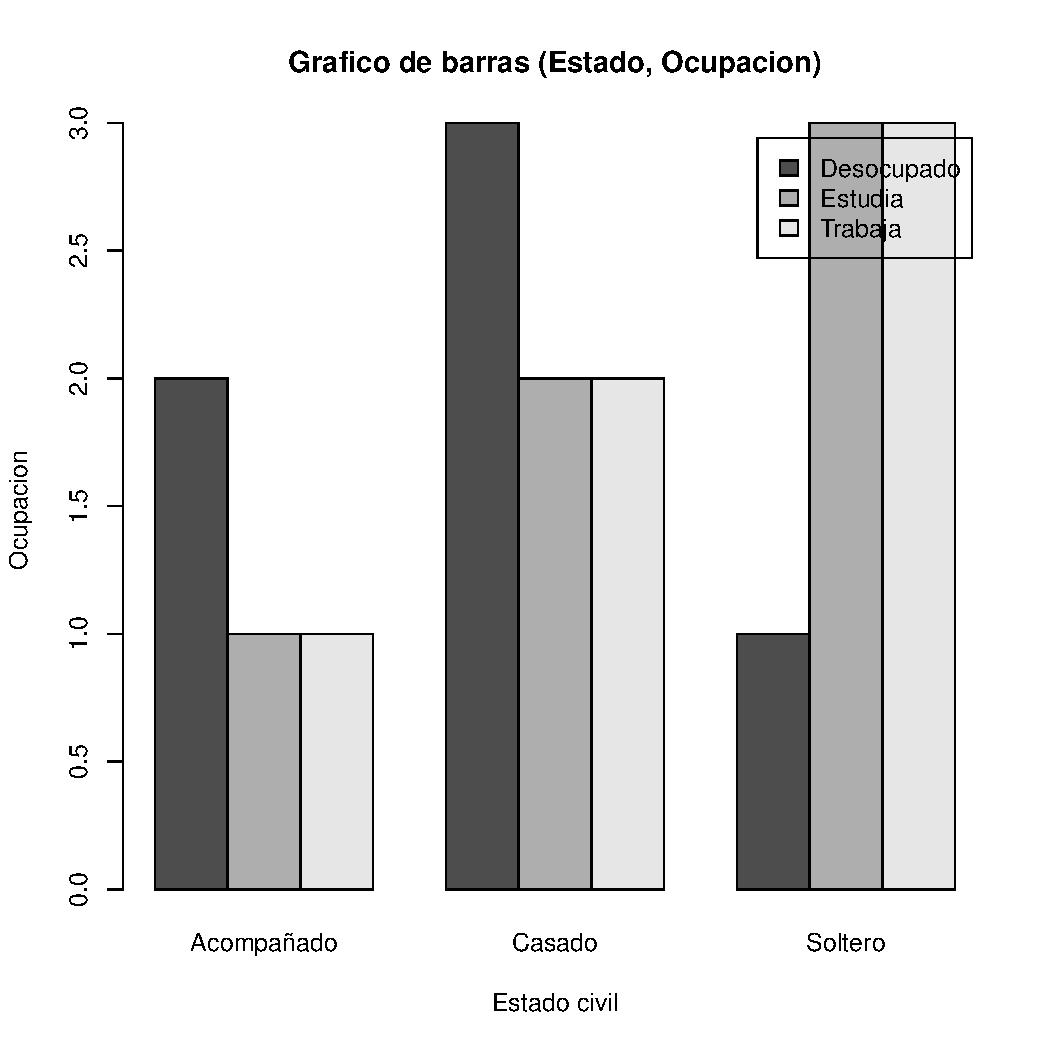
\includegraphics[width=\maxwidth]{figure/unnamed-chunk-1-2} 
\begin{kframe}\begin{alltt}
\hlstd{h} \hlkwb{<-} \hlkwd{hist}\hlstd{(X,} \hlkwc{breaks}\hlstd{=}\hlkwd{c}\hlstd{(limites[}\hlnum{1}\hlstd{]}\hlopt{-}\hlstd{a, limites, limites[k}\hlopt{+}\hlnum{1}\hlstd{]}\hlopt{+}\hlstd{a),} \hlkwc{freq} \hlstd{=} \hlnum{TRUE}\hlstd{,}
\hlkwc{probability}\hlstd{=}\hlnum{FALSE}\hlstd{,} \hlkwc{include.lowest}\hlstd{=}\hlnum{FALSE}\hlstd{,}\hlkwc{right}\hlstd{=}\hlnum{TRUE}\hlstd{,}
\hlkwc{main} \hlstd{=} \hlstr{"Poligono de frecuencias"}\hlstd{,}\hlkwc{col}\hlstd{=}\hlstr{"lightyellow"}\hlstd{,} \hlkwc{lty}\hlstd{=}\hlnum{1}\hlstd{,} \hlkwc{border}\hlstd{=}\hlstr{"purple"}\hlstd{,} \hlkwc{xlab}\hlstd{=}\hlstr{"
Notas de aspirantes"}\hlstd{,} \hlkwc{ylab}\hlstd{=}\hlstr{"Frecuencia (fi)"}\hlstd{,} \hlkwc{axes}\hlstd{=}\hlnum{TRUE}\hlstd{,} \hlkwc{labels}\hlstd{=}\hlnum{FALSE}\hlstd{)}
\hlkwd{text}\hlstd{(h}\hlopt{$}\hlstd{mids, h}\hlopt{$}\hlstd{density, h}\hlopt{$}\hlstd{counts,} \hlkwc{adj}\hlstd{=}\hlkwd{c}\hlstd{(}\hlnum{0.5}\hlstd{,} \hlopt{-}\hlnum{0.5}\hlstd{),} \hlkwc{col}\hlstd{=}\hlstr{"red"}\hlstd{)}
\hlkwd{rug}\hlstd{(}\hlkwd{jitter}\hlstd{(X))} \hlcom{# adiciona marcas de los datos}
\hlstd{vCi} \hlkwb{<-} \hlkwd{c}\hlstd{(h}\hlopt{$}\hlstd{mids[}\hlnum{1}\hlstd{]}\hlopt{-}\hlstd{a, h}\hlopt{$}\hlstd{mids, h}\hlopt{$}\hlstd{mids[k}\hlopt{+}\hlnum{1}\hlstd{]}\hlopt{+}\hlstd{a); vCi}
\end{alltt}
\begin{verbatim}
##  [1] 2.292 2.660 3.030 3.399 3.768 4.136 4.505 4.875 5.244 5.613 5.613
\end{verbatim}
\begin{alltt}
\hlstd{vfi} \hlkwb{<-} \hlkwd{c}\hlstd{(}\hlnum{0}\hlstd{, h}\hlopt{$}\hlstd{counts,} \hlnum{0}\hlstd{); vfi}
\end{alltt}
\begin{verbatim}
##  [1]  0  0  9  8 10 12  8  7  5  1  0
\end{verbatim}
\begin{alltt}
\hlkwd{lines}\hlstd{(vCi, vfi,} \hlkwc{col}\hlstd{=}\hlstr{"blue"}\hlstd{,} \hlkwc{type}\hlstd{=}\hlstr{"l"}\hlstd{)}
\end{alltt}
\end{kframe}
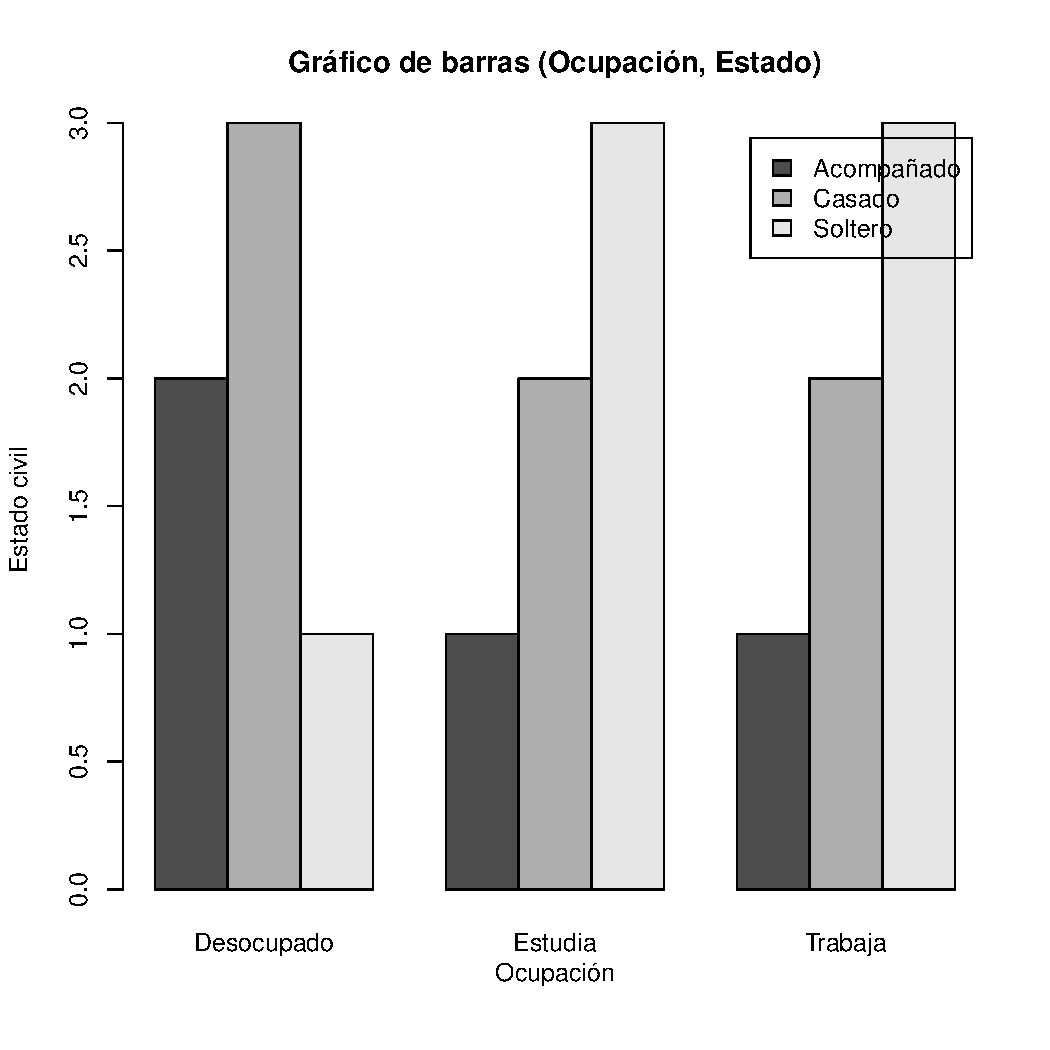
\includegraphics[width=\maxwidth]{figure/unnamed-chunk-1-3} 
\begin{kframe}\begin{alltt}
\hlstd{Fia} \hlkwb{<-} \hlkwd{c}\hlstd{(}\hlnum{0}\hlstd{, Fi); Fia}
\end{alltt}
\begin{verbatim}
## [1]  0  9 17 27 39 47 54 59
\end{verbatim}
\begin{alltt}
\hlkwd{plot}\hlstd{(limites, Fia,} \hlkwc{type} \hlstd{=} \hlstr{"p"}\hlstd{,} \hlkwc{pch}\hlstd{=}\hlnum{1}\hlstd{,} \hlkwc{col} \hlstd{=} \hlstr{"blue"}\hlstd{,} \hlkwc{main}\hlstd{=}\hlstr{"Ojiva ascendente"}\hlstd{,}
\hlkwc{xlab}\hlstd{=}\hlstr{"Notas de aspirantes"}\hlstd{,} \hlkwc{ylab}\hlstd{=}\hlstr{"Frecuencia acumulada (Fi)"}\hlstd{)}
\hlkwd{text}\hlstd{(limites, h}\hlopt{$}\hlstd{density, Fia,} \hlkwc{adj}\hlstd{=}\hlkwd{c}\hlstd{(}\hlnum{0.5}\hlstd{,} \hlopt{-}\hlnum{0.5}\hlstd{),} \hlkwc{col}\hlstd{=}\hlstr{"red"}\hlstd{)}
\hlkwd{lines}\hlstd{(limites, Fia,} \hlkwc{col}\hlstd{=}\hlstr{"black"}\hlstd{,} \hlkwc{type}\hlstd{=}\hlstr{"l"}\hlstd{)}
\end{alltt}
\end{kframe}
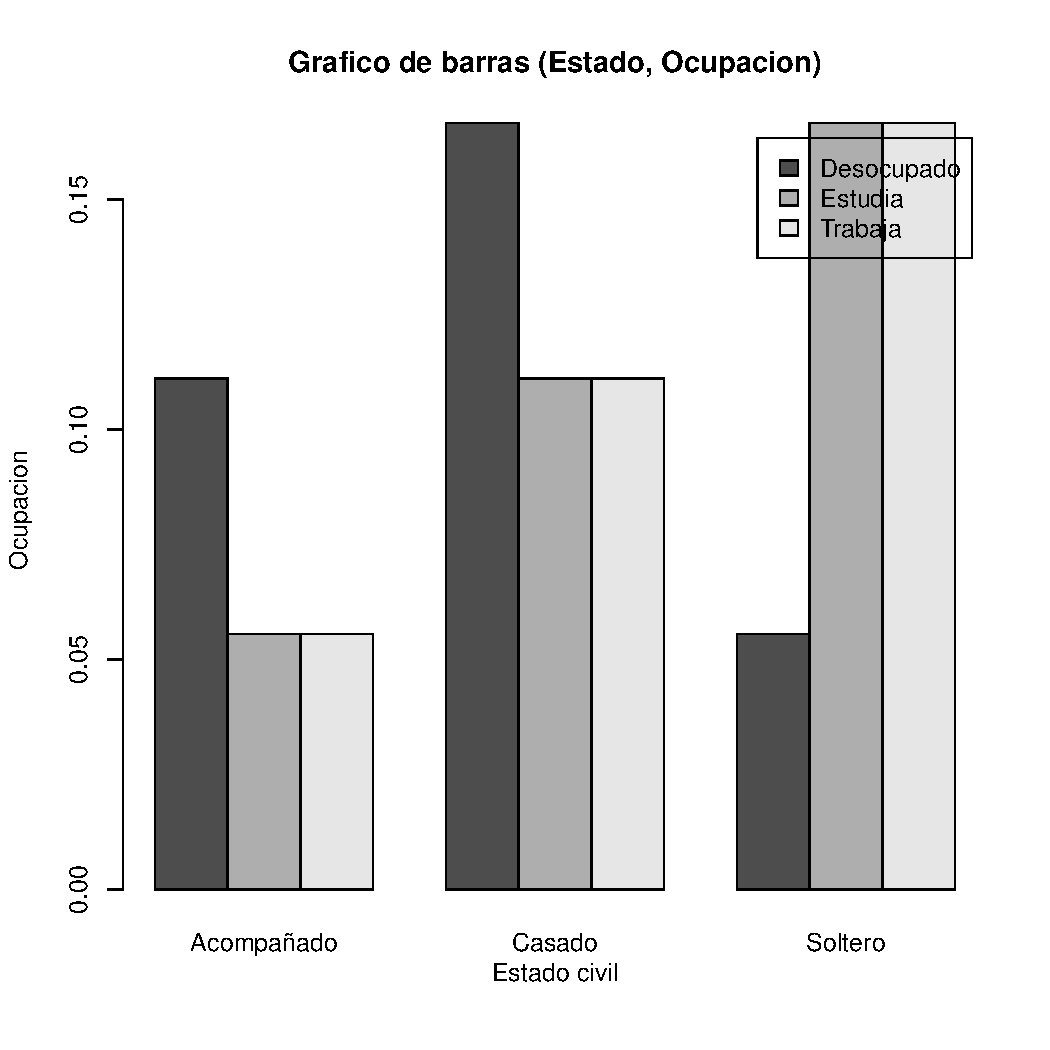
\includegraphics[width=\maxwidth]{figure/unnamed-chunk-1-4} 
\begin{kframe}\begin{alltt}
\hlcom{#Calcula los principales estadadisticos descriptivos de la variable}
\hlcom{# Calcula la moda, ya que el R no proporciona una función para eso.}
\hlkwd{options}\hlstd{(}\hlkwc{digits}\hlstd{=}\hlnum{4}\hlstd{)}
\hlkwa{for}\hlstd{(i} \hlkwa{in} \hlnum{1}\hlopt{:}\hlstd{k)} \hlkwa{if} \hlstd{(fi[i]} \hlopt{==} \hlkwd{max}\hlstd{(fi))} \hlkwa{break}\hlstd{()}
\hlkwa{if}\hlstd{(i} \hlopt{>} \hlnum{1}\hlstd{) moda} \hlkwb{<-} \hlstd{limites[i]}\hlopt{+}\hlstd{((fi[i]}\hlopt{-}\hlstd{fi[i}\hlopt{-}\hlnum{1}\hlstd{])}\hlopt{/}\hlstd{((fi[i]}\hlopt{-}\hlstd{fi[i}\hlopt{-}\hlnum{1}\hlstd{])}\hlopt{+}\hlstd{(fi[i]}\hlopt{-}\hlstd{fi[i}\hlopt{+}\hlnum{1}\hlstd{]) ))}\hlopt{*}\hlstd{a} \hlkwa{else}  \hlstd{moda} \hlkwb{<-} \hlstd{limites[i]}\hlopt{+}\hlstd{(fi[i]}\hlopt{/}\hlstd{(fi[i]}\hlopt{+}\hlstd{(fi[i]}\hlopt{-}\hlstd{fi[i}\hlopt{+}\hlnum{1}\hlstd{])))}\hlopt{*}\hlstd{a}
\hlstd{moda}
\end{alltt}
\begin{verbatim}
## [1] 4.075
\end{verbatim}
\begin{alltt}
\hlcom{# Calcula los cuartiles: Q1, Q2, Q3}
\hlstd{Q} \hlkwb{<-} \hlnum{1}\hlopt{:}\hlnum{3}
\hlkwa{for}\hlstd{(v} \hlkwa{in} \hlnum{1}\hlopt{:}\hlnum{3}\hlstd{)} \hlkwa{for}\hlstd{(i} \hlkwa{in} \hlnum{1}\hlopt{:}\hlstd{k)} \hlkwa{if} \hlstd{(Fi[i]} \hlopt{>} \hlstd{(v}\hlopt{*}\hlnum{25}\hlopt{*}\hlstd{n)}\hlopt{/}\hlnum{100}\hlstd{)}
\hlstd{\{}
\hlstd{Q[v]} \hlkwb{<-} \hlstd{limites[i]}\hlopt{+}\hlstd{(((}\hlnum{25}\hlopt{*}\hlstd{v}\hlopt{*}\hlstd{n}\hlopt{/}\hlnum{100}\hlstd{)}\hlopt{-}\hlstd{Fi[i}\hlopt{-}\hlnum{1}\hlstd{])}\hlopt{/}\hlstd{fi[i])}\hlopt{*}\hlstd{a}
\hlkwa{break}
\hlstd{\}}
\hlstd{Q}
\end{alltt}
\begin{verbatim}
## [1] 3.491 4.044 4.598
\end{verbatim}
\begin{alltt}
\hlcom{#Calcula los principales estadisticos.}
\hlstd{estadisticos} \hlkwb{<-} \hlkwd{rbind}\hlstd{(}\hlkwc{media}\hlstd{=}\hlkwd{sum}\hlstd{(tabEstad}\hlopt{$}\hlstd{cifi)}\hlopt{/}\hlstd{n,} \hlkwc{moda}\hlstd{=moda,} \hlkwc{Q1}\hlstd{=Q[}\hlnum{1}\hlstd{],} \hlkwc{Q2}\hlstd{=Q[}\hlnum{2}\hlstd{],} \hlkwc{Q3}\hlstd{=Q[}\hlnum{3}\hlstd{],}
\hlkwc{rango}\hlstd{=}\hlkwd{max}\hlstd{(X)}\hlopt{-}\hlkwd{min}\hlstd{(X),} \hlkwc{varianza}\hlstd{=}\hlkwd{sum}\hlstd{(tabEstad}\hlopt{$}\hlstd{ciMedia2fi)}\hlopt{/}\hlstd{n,}
\hlkwc{Desviacion}\hlstd{=}\hlkwd{sqrt}\hlstd{(}\hlkwd{sum}\hlstd{(tabEstad}\hlopt{$}\hlstd{ciMedia2fi)}\hlopt{/}\hlstd{n),}
\hlkwc{CoeficienteVariacion}\hlstd{=}\hlkwd{sqrt}\hlstd{(}\hlkwd{sum}\hlstd{(tabEstad}\hlopt{$}\hlstd{ciMedia2fi)}\hlopt{/}\hlstd{n)}\hlopt{/}\hlstd{(}\hlkwd{sum}\hlstd{(tabEstad}\hlopt{$}\hlstd{cifi)}\hlopt{/}\hlstd{n),}
\hlkwc{CAfisher}\hlstd{=(}\hlkwd{sum}\hlstd{(tabEstad}\hlopt{$}\hlstd{ciMedia3fi)}\hlopt{/}\hlstd{n)}\hlopt{/}\hlkwd{sqrt}\hlstd{(}\hlkwd{sum}\hlstd{(tabEstad}\hlopt{$}\hlstd{ciMedia2fi)}\hlopt{/}\hlstd{n)}\hlopt{^}\hlnum{3}\hlstd{,}
\hlkwc{CoeficienteCurtosis}\hlstd{=((}\hlkwd{sum}\hlstd{(tabEstad}\hlopt{$}\hlstd{ciMedia4fi)}\hlopt{/}\hlstd{n)}\hlopt{/}\hlkwd{sqrt}\hlstd{(}\hlkwd{sum}\hlstd{(tabEstad}\hlopt{$}\hlstd{ciMedia2fi)}\hlopt{/}\hlstd{n)}\hlopt{^}\hlnum{4}\hlstd{)}\hlopt{-}\hlnum{3}\hlstd{)}
\end{alltt}


{\ttfamily\noindent\bfseries\color{errorcolor}{\#\# Error in rbind(media = sum(tabEstad\$cifi)/n, moda = moda, Q1 = Q[1], Q2 = Q[2], : objeto 'tabEstad' no encontrado}}\begin{alltt}
\hlstd{estadisticos}
\end{alltt}


{\ttfamily\noindent\bfseries\color{errorcolor}{\#\# Error in eval(expr, envir, enclos): objeto 'estadisticos' no encontrado}}\begin{alltt}
\hlcom{# Grafico de cajas}
\hlkwd{boxplot}\hlstd{(X,} \hlkwc{main}\hlstd{=}\hlstr{"Gráfico de caja"}\hlstd{,} \hlkwc{xlab}\hlstd{=}\hlstr{"Notas"}\hlstd{,} \hlkwc{notch}\hlstd{=}\hlnum{FALSE}\hlstd{,}
\hlkwc{data}\hlstd{=}\hlkwd{parent.frame}\hlstd{(),} \hlkwc{plot}\hlstd{=}\hlnum{TRUE}\hlstd{,} \hlkwc{border}\hlstd{=}\hlstr{"red"}\hlstd{,} \hlkwc{col}\hlstd{=}\hlstr{"yellow"}\hlstd{,}\hlkwc{horizontal}\hlstd{=}\hlnum{TRUE}\hlstd{)}
\end{alltt}
\end{kframe}
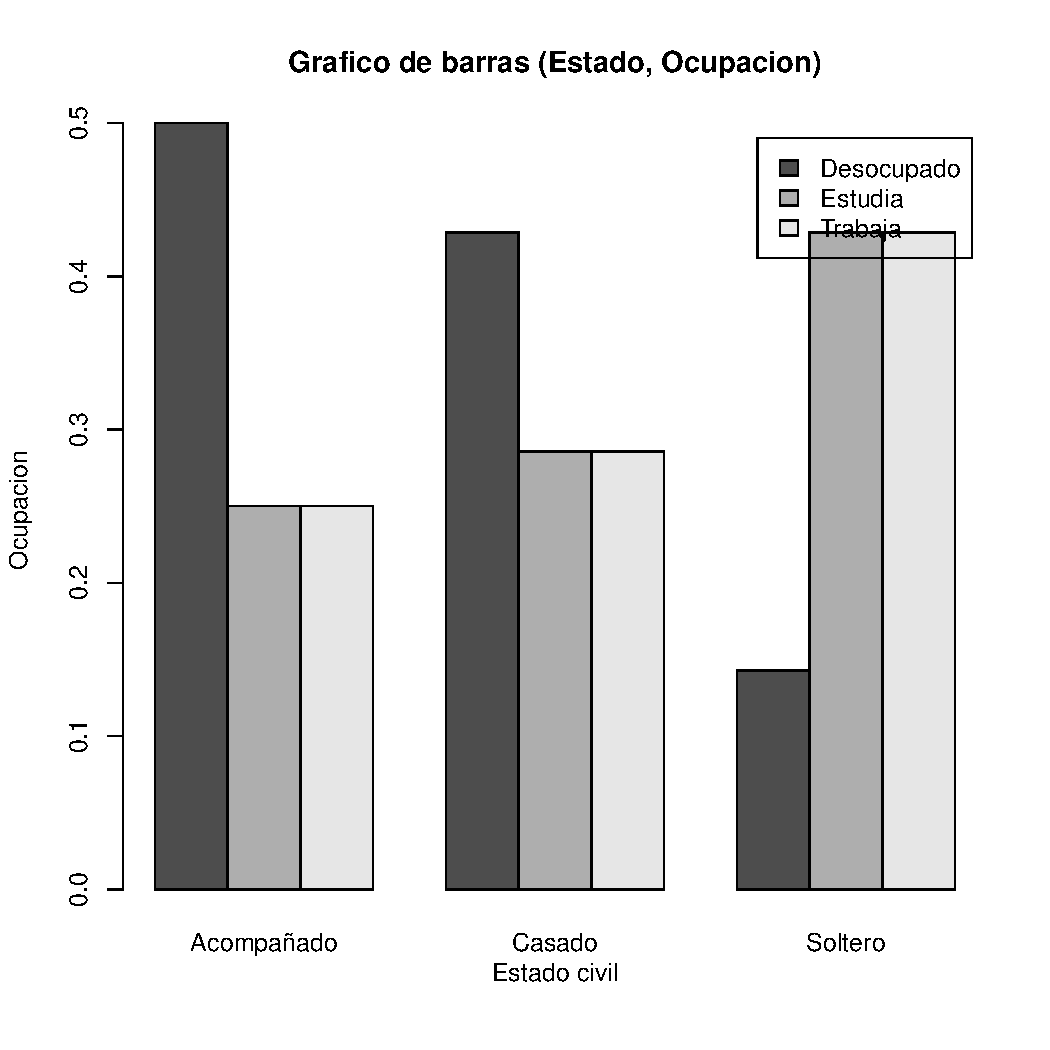
\includegraphics[width=\maxwidth]{figure/unnamed-chunk-1-5} 
\begin{kframe}\begin{alltt}
\hlcom{#Observacion: en la función boxplot(), s�? plot es FALSE se produce un resumen de los valores (los cinco numeros).}


\hlkwd{windows}\hlstd{()}
\hlkwd{boxplot}\hlstd{(X,} \hlkwc{main}\hlstd{=}\hlstr{"Grafico de caja"}\hlstd{,} \hlkwc{xlab}\hlstd{=}\hlstr{"X = Notas"}\hlstd{,} \hlkwc{notch}\hlstd{=}\hlnum{TRUE}\hlstd{,}
\hlkwc{data}\hlstd{=}\hlkwd{parent.frame}\hlstd{(),} \hlkwc{plot}\hlstd{=}\hlnum{TRUE}\hlstd{,} \hlkwc{border}\hlstd{=}\hlstr{"red"}\hlstd{,} \hlkwc{col}\hlstd{=}\hlstr{"yellow"}\hlstd{,}\hlkwc{horizontal}\hlstd{=}\hlnum{TRUE}\hlstd{)}

\hlkwd{par}\hlstd{(}\hlkwc{mfrow}\hlstd{=}\hlkwd{c}\hlstd{(}\hlnum{1}\hlstd{,}\hlnum{2}\hlstd{))} \hlcom{# Divide la ventana grafica en dos partes (1 fila, 2 columnas)}
\hlkwd{mtext}\hlstd{(}\hlkwc{side}\hlstd{=}\hlnum{3}\hlstd{,} \hlkwc{line}\hlstd{=}\hlnum{0}\hlstd{,} \hlkwc{cex}\hlstd{=}\hlnum{2}\hlstd{,} \hlkwc{outer}\hlstd{=T,} \hlstr{"Titulo para Toda la Pagina"}\hlstd{)}
\end{alltt}
\end{kframe}
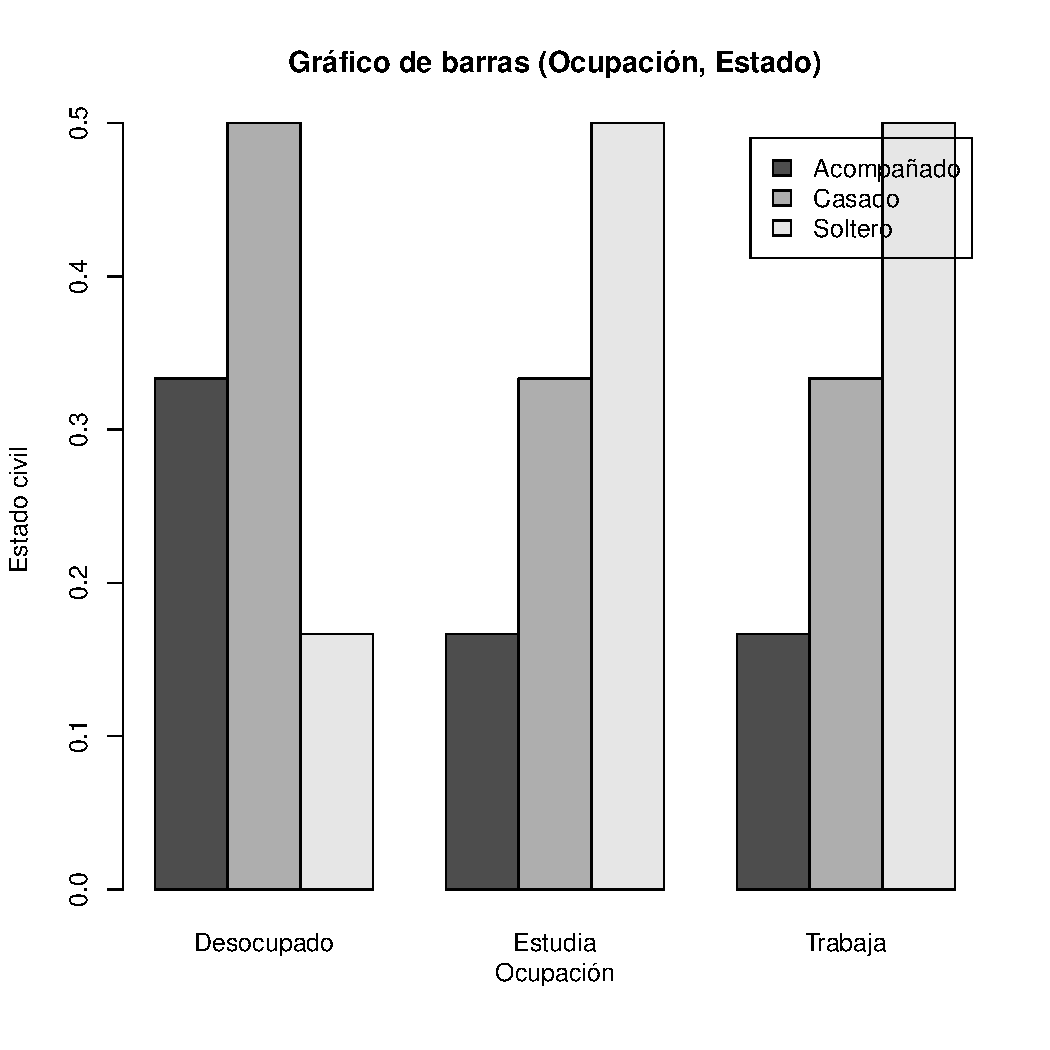
\includegraphics[width=\maxwidth]{figure/unnamed-chunk-1-6} 
\begin{kframe}\begin{alltt}
\hlkwd{hist}\hlstd{(X);} \hlkwd{boxplot}\hlstd{(X)}

\hlcom{#Calcula los principales estad�sticos descriptivos de la variable}
\hlcom{# Calcula la moda, ya que el R no proporciona una funci�n para eso.}
\hlkwd{options}\hlstd{(}\hlkwc{digits}\hlstd{=}\hlnum{4}\hlstd{)}
\hlkwa{for}\hlstd{(i} \hlkwa{in} \hlnum{1}\hlopt{:}\hlstd{k)} \hlkwa{if} \hlstd{(fi[i]} \hlopt{==} \hlkwd{max}\hlstd{(fi))} \hlkwa{break}\hlstd{()}
\hlkwa{if}\hlstd{(i} \hlopt{>} \hlnum{1}\hlstd{) moda} \hlkwb{<-} \hlstd{limites[i]}\hlopt{+}\hlstd{((fi[i]}\hlopt{-}\hlstd{fi[i}\hlopt{-}\hlnum{1}\hlstd{])}\hlopt{/}\hlstd{((fi[i]}\hlopt{-}\hlstd{fi[i}\hlopt{-}\hlnum{1}\hlstd{])}\hlopt{+}\hlstd{(fi[i]}\hlopt{-}\hlstd{fi[i}\hlopt{+}\hlnum{1}\hlstd{]) ))}\hlopt{*}\hlstd{a}
\hlstd{moda} \hlkwb{<-} \hlstd{limites[i]}\hlopt{+}\hlstd{(fi[i]}\hlopt{/}\hlstd{(fi[i]}\hlopt{+}\hlstd{(fi[i]}\hlopt{-}\hlstd{fi[i}\hlopt{+}\hlnum{1}\hlstd{])))}\hlopt{*}\hlstd{a}
\hlstd{moda}
\end{alltt}
\begin{verbatim}
## [1] 4.229
\end{verbatim}
\begin{alltt}
\hlcom{#Varios gr�ficos en una misma ventana}
\hlkwd{par}\hlstd{(}\hlkwc{mfrow}\hlstd{=}\hlkwd{c}\hlstd{(}\hlnum{1}\hlstd{,}\hlnum{2}\hlstd{))} \hlcom{# Divide la ventana gr�fica en dos partes (1 fila, 2 columnas)}
\hlkwd{mtext}\hlstd{(}\hlkwc{side}\hlstd{=}\hlnum{3}\hlstd{,} \hlkwc{line}\hlstd{=}\hlnum{0}\hlstd{,} \hlkwc{cex}\hlstd{=}\hlnum{2}\hlstd{,} \hlkwc{outer}\hlstd{=T,} \hlstr{"Titulo para Toda la P�gina"}\hlstd{)}
\end{alltt}
\end{kframe}
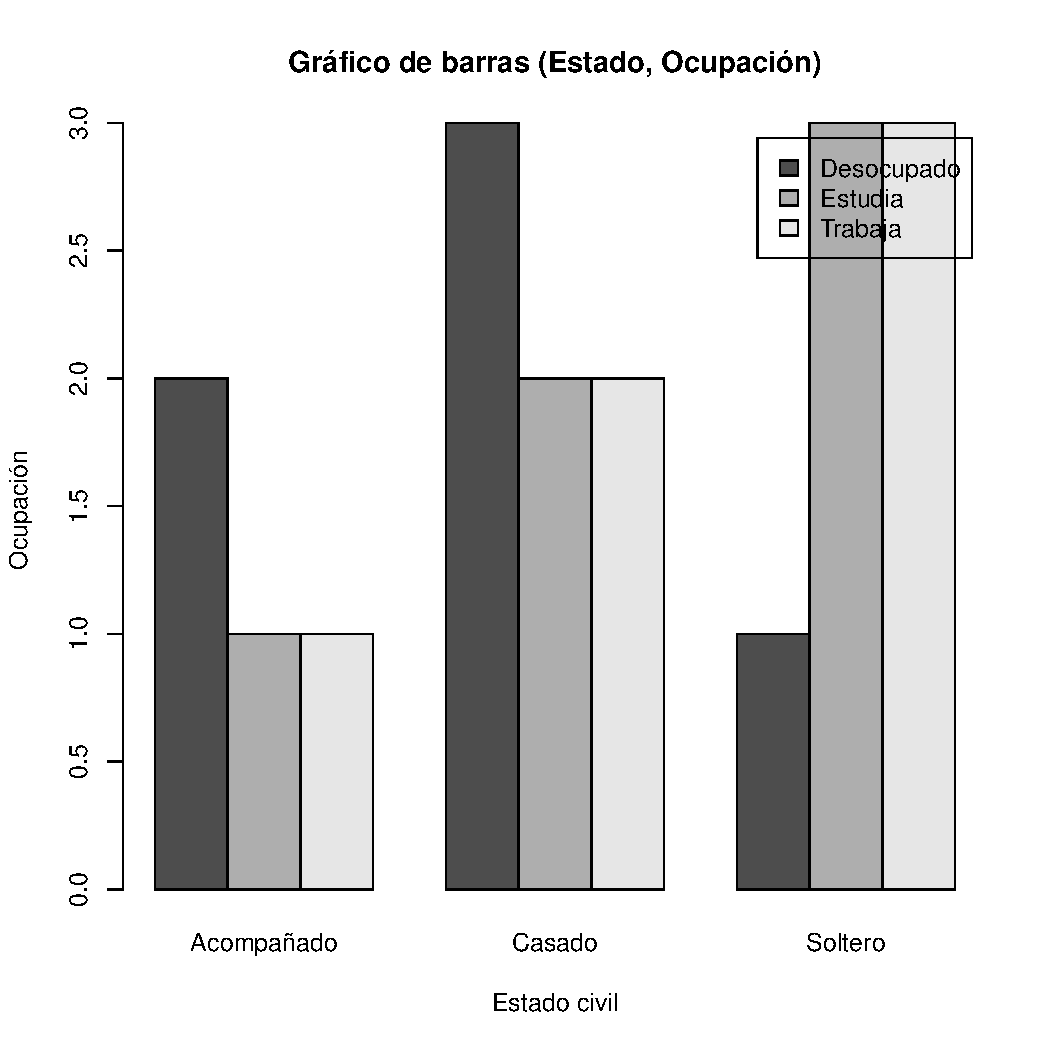
\includegraphics[width=\maxwidth]{figure/unnamed-chunk-1-7} 
\begin{kframe}\begin{alltt}
\hlkwd{hist}\hlstd{(X);} \hlkwd{boxplot}\hlstd{(X)}
\end{alltt}
\end{kframe}
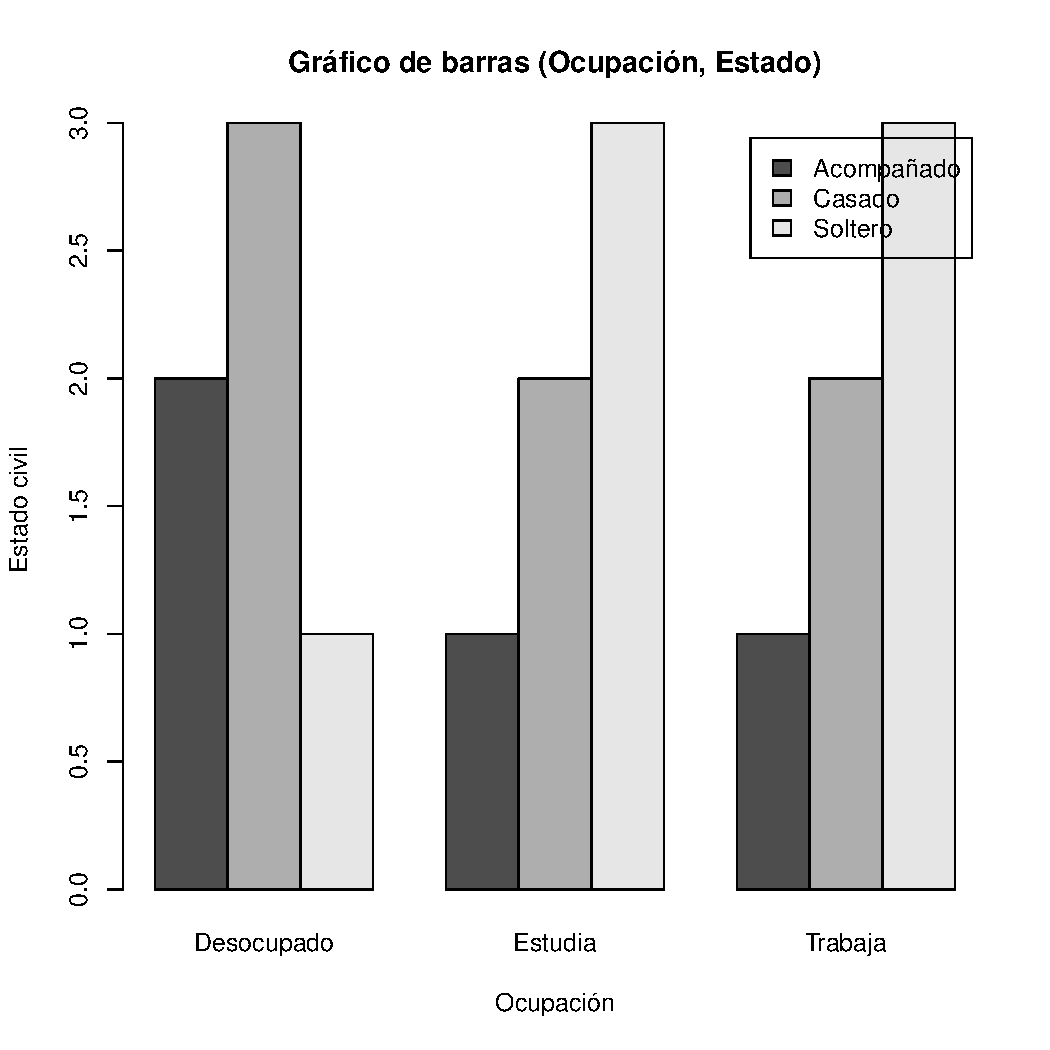
\includegraphics[width=\maxwidth]{figure/unnamed-chunk-1-8} 

\end{knitrout}
\end{document}
